\documentclass[12pt,letterpaper]{article}

%Packages
% \usepackage{textcomp}
% \usepackage{latexsym}
% \usepackage{url}
% \usepackage{amssymb}
% \usepackage{amsmath}
% \usepackage{mathtools}
% \usepackage{bm}
% \usepackage{array}
% \usepackage[version=3]{mhchem}
% \usepackage{ifthen}
% \usepackage{amsthm}
% \usepackage{amstext}
% \usepackage{enumerate}
% \usepackage{dcolumn}

\usepackage{scicite}
\usepackage{epsfig}
\usepackage{graphicx}
\usepackage{caption}
\usepackage{hyperref}
\usepackage{lineno}
\usepackage{pdflscape}
\usepackage{mathtools}
\usepackage[osf]{mathpazo}
\usepackage{fullpage}
\usepackage{float}
\usepackage{xr} %linking to supplementaries
\usepackage{setspace} % double spacing
\externaldocument{supplementaries}

\pagenumbering{arabic}


%---------------------------------------------
%
%       START
%
%---------------------------------------------

\begin{document}
%Running head
\begin{flushright}
Version dated: \today
\end{flushright}

\bigskip
\begin{center}

\noindent{\Large \bf Innovation and elaboration on the avian tree of life}
\bigskip

% Short title: Innovation and elaboration in birds

% One sentence summary: Species elaborate; clades innovate, reconciling evolutionary theory from micro- to megaevolutionary scales.


\noindent {\normalsize \sc
Thomas Guillerme$^{1,*}$, 
Jen A. Bright$^{2}$,
Christopher R. Cooney${^1}$,
Emma C. Hughes${^1}$,
% Zoe K. Varley${^3}$,
Natalie Cooper$^{3,+}$,
Andrew P. Beckerman$^{1,+}$,
and Gavin H. Thomas$^{1,4,+}$}\\
\noindent {\small \it 
$^1$School of Biosciences, University of Sheffield, Sheffield, S10 2TN, United Kingdom.\\
$^2$School of Natural Science, University of Hull, Hull, HU6 7RX, United Kingdom.\\
$^3$Natural History Museum, Cromwell Road, London, SW7 5BD, United Kingdom.\\
$^4$Bird Group, Department of Life Sciences, the Natural History Museum at Tring, Tring, United Kingdom.\\}

\end{center}
\bigskip
\noindent{*\bf Corresponding author:} \textit{guillert@tcd.ie}; \noindent{+\bf contributed equally.}\\
% \vspace{1in}

%Line numbering
\modulolinenumbers[1]
\linenumbers

\doublespacing

%---------------------------------------------
%
%       ABSTRACT
%
%---------------------------------------------

\noindent (Keywords: macroevolution, elaboration, innovation, variance-covariance matrices, line of least resistance, GLMM)\\

\section*{Abstract}

Widely documented, megaevolutionary jumps in diversity continue to perplex researchers because it remains unclear whether these dramatic changes can emerge from microevolutionary processes.
Here we reconcile major changes in phenotypic diversity at macroevolutionary scales with gradual microevolutionary change using new multi-trait models to evaluate the magnitude and distribution of elaboration and innovation in the evolution of bird beaks.
We find that elaboration dominates at macroevolutionary scales whereas innovation becomes more prominent at megaevolutionary scales.
Indeed, the major axis of phenotypic change among species at megaevolutionary scales is an emergent property of innovation across clades.
Our analyses suggest that the reorientation of phenotypes via innovation is a ubiquitous route for divergence that can arise through gradual change alone, opening up new avenues for evolution to explore.

\section*{Introduction}

Evolutionary theory predicts that over short, microevolutionary, timescales phenotypic evolution will tend to follow evolutionary lines of genetic least resistance \cite{schluter1996adaptive}.
Over longer timescales, the evolutionary line of least resistance is analogous to the major axis of phenotypic variation \cite{marroig2005size,renaud2006conserved,fasanelli2022allometry}.
Numerous studies show that phenotypic divergence is biased along the evolutionary line of least resistance, and therefore reflects the major axis of phenotypic variation, over 1-2 million year timescales \cite{marroig2005size, mcglothlin2018adaptive, tsuboi2018}.
Recent evidence suggests that this stability can even extend over macroevolutionary timescales spanning tens of millions of years \cite{mcglothlin2018adaptive}.
However, while the evolutionary line of genetic least resistance explicitly reflects genetic constraints, the macroevolutionary major axis of phenotypic variation is an emergent property of genomic and developmental constraints interacting with selection on a moving adaptive landscape \cite{jones2004evolution,BurinWhales}.
The widespread evidence of major shifts in phenotypes across the tree of life \cite{venditti2011multiple,pagel2022general,khabbazian2016fast,cooney2017mega,smaers2021evolution,goswami2022} suggests a conflict in the direction of phenotypic evolution across scales where macroevolutionary divergence away from the major axis of phenotypic variation results in megaevolutionary divergence leading to distinct phenotypes and/or directions of evolution.
Resolving this conflict requires an understanding of the balance between deep-time reorientation of phenotypic major axes of evolution among clades and the directions of evolution of species within clades.


Endler \textit{et al}. \cite{endler2005animal}, writing in the specific context of signal evolution, describe two routes to phenotypic novelty that we suggest can help to illuminate this challenge.
Specifically, Endler \textit{et al}. refer to evolution of new phenotypes along the same major axis of phenotypic variation as \textit{elaboration}.
This is akin to phenotypic divergence among species following lines of least resistance, and, by definition, would be expected to be a major driver of phenotypic evolution.
In contrast, they refer to evolution away from the major axis of phenotypic variation, either in random directions or along limited axes, as \textit{innovation} \cite{endler2005animal}.
Relative to elaboration, innovation may be more likely to generate phenotypic novelty, but this need not be synonymous with being a primary driver of phenotypic diversity at broad scales.
These core concepts can now be defined using robust multivariate statistics about trait covariance applied at multiple phylogenetic scales and provide a powerful theoretical framework with which to study macro- to mega-evolutionary divergence and in particular to determine the relative importance of:
i) idiosyncratic species-level innovation against clade-level innovation (i.e. reorientation of the directions of phenotypic variation),
and ii) evolution along versus away from major axes of phenotypic variation.
The contributions of these multivariate, evolutionary pathways are poorly-known despite their importance for understanding the origins of diversity from macro- to mega-evolutionary scales. 
Here we estimate for the first time, using novel statistical methods, the relative contribution of elaboration and innovation to the remarkable global radiation and diversity of birds beaks.
 
\section*{Modelling nested trait covariances}
Addressing the relative contributions of elaboration and innovation to the origins of biodiversity in deep-time requires
1) large, multivariate datasets to allow exploration of trait covariances at different scales,
2) reliable and efficient computational methods to estimate the major axes of phenotypic variation,
and 3) a set of mathematical tools that can estimate degrees of elaboration and innovation at any scale.
To meet the first challenge we use an eight-dimensional beak shape morphospace based on a geometric, morphometric dataset of 8748 species of birds (described in \cite{hughes2022global}).
To meet the other two challenges we introduce a novel analytical pipeline for measuring elaboration and innovation at the species-level and clade-level (Fig.S\ref{Fig:cheat_sheet} and S\ref{Fig:mcmcmcglmm}).
To estimate the major axis of phenotypic variation we fit Bayesian phylogenetic generalised linear mixed model (pGLMM) models with beak shape as an eight-dimensional response variable \cite{MCMCglmm}.
From the posterior distribution of the variance-covariance matrix at any scale, the major axis can be identified from the leading eigenvector of the variance-covariance matrix.
We can estimate levels of elaboration and innovation based on that major axis of phenotypic variation (see Methods).
We regard the major axis of phenotypic variation as a deep-time analogue of the microevolutionary \textbf{G} matrix \cite{robinson2013quantifying} and posit that it represents the line of least evolutionary resistance, capturing the effects of historical contingency on multivariate evolution.
The major axis of phenotypic variation can be defined at any phylogenetic scale (i.e. for all species in the phylogeny, or for all species within any clade).
To assess the roles of elaboration and innovation across scales we fit our pGLMMs as nested models in which we define variance-covariance matrices, and therefore major axes of phenotypic variation, for
i) the entire phylogeny of all species included in the data (hereafter the global phylogenetic level),
ii) all species within each of nine clades mapping approximately to super-orders (the super-order level),
and iii) all species within each of 27 clades mapping to taxonomic orders (the order level).
These nested partitions of multivariate trait space provide the basis for all subsequent quantitative estimates of elaboration and innovation at multiple scales.

\section*{Elaboration dominates species-level divergence}
We tested the expectation, derived from adaptive radiation theory, that species divergence is biased along evolutionary lines of least resistance by calculating species-specific measures of innovation and elaboration.
If microevolutionary lines of least resistance are stable then we expect that species fall on a conserved major axis (elaboration) rather than off the line (innovation).
To assess this we calculated the multilinear algebraic projection of each species phenotype onto three major axes of phenotypic variation (global phylogenetic, super-order, and order).
We found higher values of elaboration than innovation overall across all levels (Fig \ref{Fig:phylogeny}) and globally more elaboration and innovation at the global phylogenetic and super-order levels compared to the order level.
Phylogenetic distributions of innovation and elaboration broadly hold whether comparisons are made at the order, super-order, or global phylogenetic level (Fig. \ref{Fig:phylogeny})%{#fig_correlations}),%TODO: maybe add to supp?
 and in further nested analysis of the order Passeriformes (Fig. S\ref{fig_ellipses_passeriformes} and S\ref{fig_phylogeny_passeriformes}).
However, the extent of both elaboration and innovation tends to reduce as we move from global phylogenetic to within-order comparisons.
Broadly, and not surprisingly, this trend reflects the fact that species are more similar to the major axis of phenotypic variation of their close relatives than to the major axis of phenotypic variation of all birds.
The global phylogenetic major axis of phenotypic variation aligns closely with the major axis in the trait space and primarily describes variation between short, deep, and wide beaks at one extreme, and long, shallow, and narrow beaks at the other.
Our results point to the possibility that within clades the major axes of phenotypic variation follow different directions. 

Overall we found that, as expected from microevolutionary theory, elaboration is the dominant mode of divergence at the species level (Fig. \ref{Fig:phylogeny}).
We find no consistent evidence that innovation is either positively correlated, or trades-off, with elaboration. %(Fig. S{#fig_correlations}). %TODO: maybe add to supp? 
However, we observe various combinations of elaboration and innovation across birds.
Examples of high innovation and/or elaboration are often clustered within clades.
For example, compared to the global phylogenetic major axis of phenotypic variation, the Trochilidae (hummingbirds) in the order Apodiformes, have long narrow beaks and display high levels of elaboration and low innovation.
In contrast, the Bucerotiformes (hornbills), with large and deep beaks display high levels of innovation and low elaboration.
Other clades such as the Apodidae (swifts), in the order Apodiformes, and the distantly-related but convergent Hirundinidae (swallows and martins) in the order Passeriformes, have exceptionally wide beaks relative to length and display high levels of both elaboration and innovation.
The dominance of elaboration when measured at the species-level is consistent with the idea of evolution along lines of least evolutionary resistance.
The frequent phylogenetic clustering of species that elaborate, innovate, or both, highlights the likelihood that major axes of phenotypic variation are not stable among clades.
This leads us to ask; if most organisms evolve incrementally along the major axis of phenotypic variation then how can we explain the staggering diversity of species morphologies across the tree of life? 

% \begin{figure}[!htbp]
% \centering
%     \includegraphics[width=0.9\textwidth]{Figures/InnovElabTree_main_text_with_box.pdf}
% \caption{.}
% \label{Fig:phylogeny}
% \end{figure}


% \bigskip

% \noindent \textbf{Figure \ref{Fig:phylogeny}:}
% The avian phylogeny (n = 8748 species) coloured by species beak shape innovation and elaboration level.
% Blue and yellow colours on the branches of the phylogeny highlight species with relatively low distances to the global centroid of trait space whereas orange to red colours indicate high distance from the centroid.
% Innovation and elaboration scores are represented concentrically in a nested fashion with the most external pairs of circles (innovation and elaboration bands) representing comparisons for each species at the order level, then at the super-order level, and finally at the global phylogenetic level.
% The boxplots at the bottom of the figure summarise the distribution of the median innovation and elaboration values for all levels (bottom left), showing that elaboration is more common than elaboration,
% and the pooled median innovation and elaboration values for all three different levels (bottom right), showing that elaboration and innovation is more common at higher taxonomic levels than at the order level.
% We can observe an increase in the distance of species to the global centroid of trait space at deeper phylogenetic scales with greater distances generally composed of more elaboration than innovation.
% A companion plot showing further nested structure within the Passeriformes is shown in Fig. S\ref{fig_phylogeny_passeriformes}. 

\section*{Multiple routes to innovation throughout avian evolutionary history}

To investigate the conflict implied by our observations of species-level elaboration and previously reported deep-time jumps in phenotype, we measured the elaboration and innovation of different clades.
To do this we translated the major axes of phenotypic variation of each clade's (i.e. super-orders and orders) phylogenetic variance-covariance matrix onto the global phylogenetic major axis of phenotypic variation so that they shared the same origin in the shapespace.
We then used multilinear algebra to project a focal clade's major axis of phenotypic variation onto the global phylogenetic major axis of phenotypic variation (Fig.S\ref{Fig:cheat_sheet}).
We interpret the measured projection (distance onto the phylogenetic major axis of phenotypic variation) as the clade's elaboration score and the measured rejection (distance from the major axis of phenotypic variation) as the clade's innovation score.
A high innovation score indicates that the direction of evolution of a clade differs from the direction of its parent clade (e.g. the direction of evolution of an order differs from its parent super-order).
These scores were measured for each of 4000 posterior pairs of clade vs. phylogenetic variance-covariance matrix (Fig.\ref{Fig:ellipses} boxplots).
We found that for most clades the major axis of phenotypic variation is not aligned with the global phylogenetic major axis of phenotypic variation (Fig. \ref{Fig:ellipses}). 
Despite the limitations of representing eight-dimensional space in 2D, our plots of the average elliptical representation of the phenotypic variance-covariance matrix for the global phylogenetic major axis of phenotypic variation and each super-order (Fig. \ref{Fig:ellipses}a) and order (Fig. \ref{Fig:ellipses}b) highlight the striking variation in the orientation of phenotypic major axes among clades (Fig. \ref{Fig:orthogonality}).
Remarkably, more than half of the assessed clades (4/8 super-orders and 15/27 orders) displayed higher median innovation than median elaboration scores implying that, contrary to microevolutionary theory \cite{schluter1996adaptive,marroig2005size}, innovation is a more common generator of morphological diversity than elaboration in deep-time (i.e evidence at the clade scale).
However, there is substantial variation in elaboration and innovation among clades including relatively low elaboration and innovation (e.g. Cuculiformes; Fig. \ref{Fig:ellipses}), low elaboration and high innovation (e.g. Galliformes; Fig. \ref{Fig:ellipses}), high elaboration and low innovation (e.g. Coraciiformes; Fig. \ref{Fig:ellipses}), and both relatively high elaboration and innovation (e.g. Podicipediformes; Fig. \ref{Fig:ellipses}).
These patterns hold across scales including within super-orders and at finer scales within the order Passeriformes (Fig. S\ref{fig_ellipses_passeriformes}).
Our observations of heterogeneity in the orientation of the major axis of phenotypic variation among clades is further supported by consistent evidence for orthogonality of clades relative to the global phylogenetic major axis of phenotypic variation (Fig. \ref{Fig:ellipses} - Fig. \ref{Fig:orthogonality}).
The median angle of the major axis of phenotypic variation for subclades approaches orthogonality, differing from the global phylogenetic major axis of phenotypic variation by $68.14^\circ$ ($95$\% CI: $22.83^\circ$-$89.09^\circ$ - Fig. \ref{Fig:orthogonality}).
Comparisons of orientation among subclades (i.e. orders within super-orders) show similar differences (median = $47.14^\circ$; $95$\% CI: $13.64^\circ$-$87.62^\circ$ - Fig. \ref{Fig:orthogonality}), suggesting that reorientations in trait space are largely unconstrained at the megaevolutionary level and are no more likely to occur along any one axis than another.
This differs from previous inference on a subset of our data that implied generally consistent and low dimensionality within clades \cite{cooney2017mega}.
This suggests that there is no deep-time analogue of the genetic line of least resistance and that across scales there is remarkable flexibility in the routes to innovation, consistent with the idea that morphological divergence may be less constrained in deep-time than is often assumed \cite{venditti2011multiple}.

% \begin{figure}[!htbp]
% \centering
%    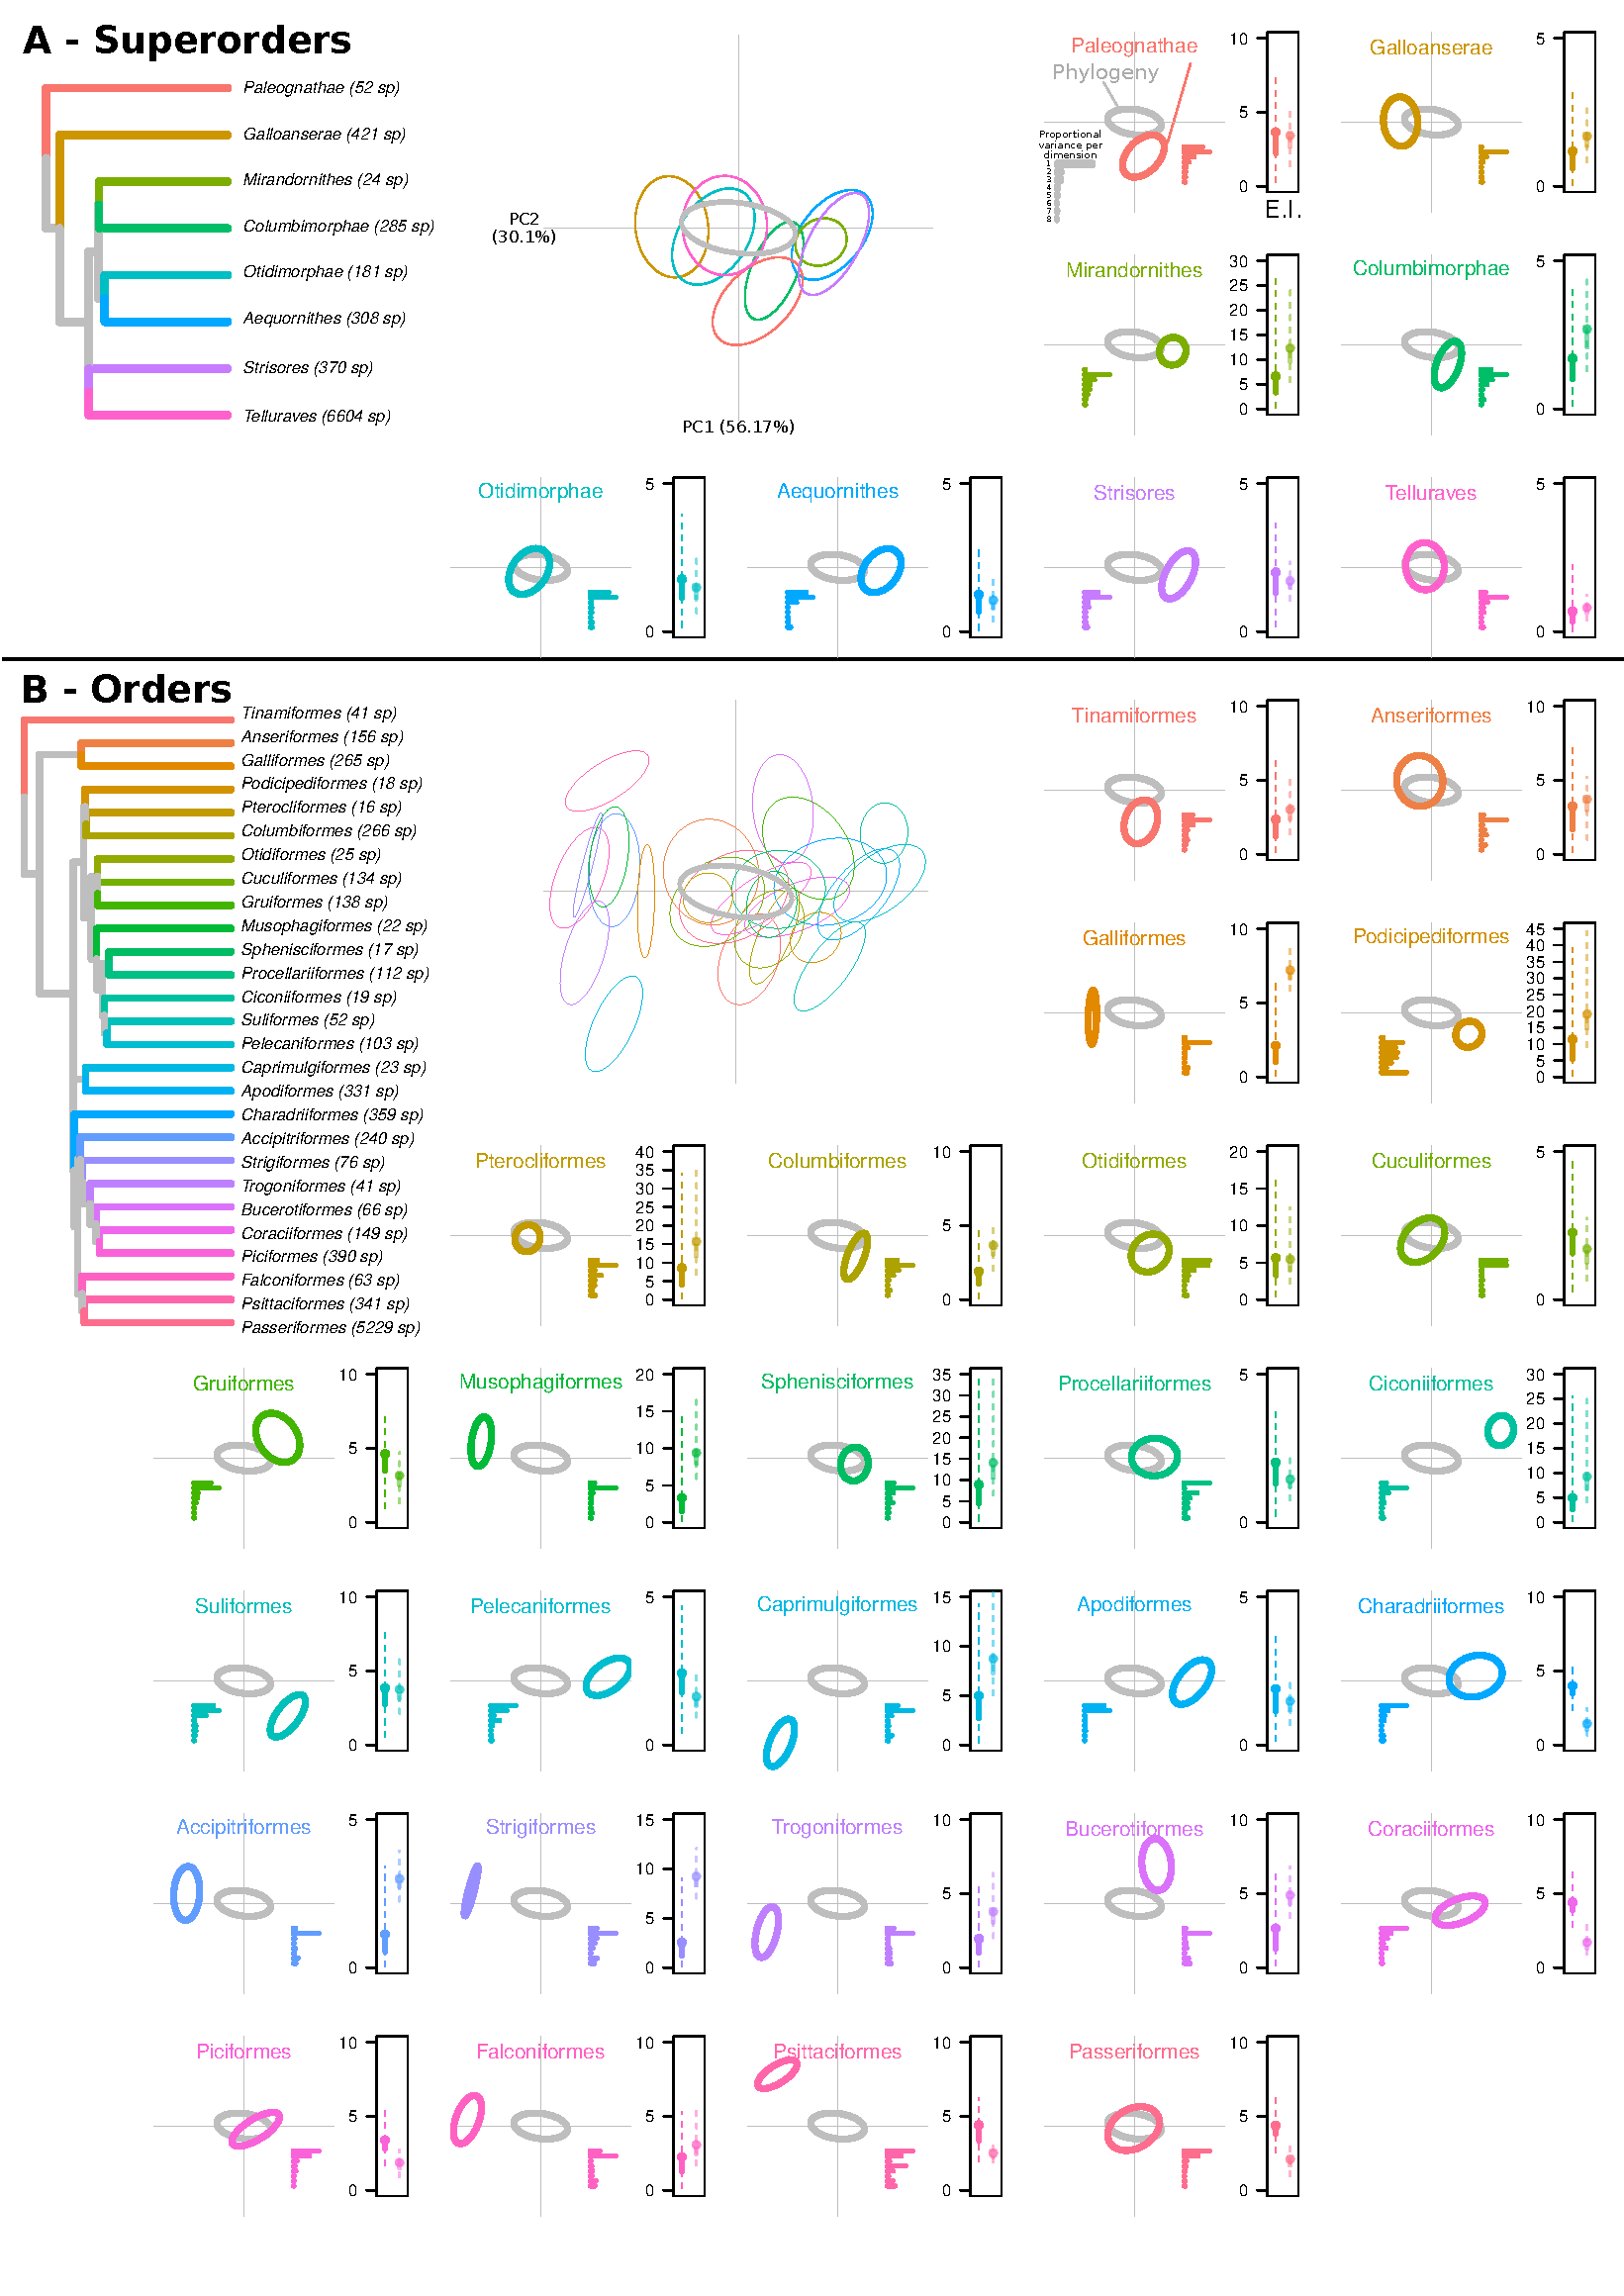
\includegraphics[width=1\textwidth]{Figures/ellipses.pdf}
% \caption{.}
% \label{Fig:ellipses}
% \end{figure}
% \bigskip

% \noindent \textbf{Figure \ref{Fig:ellipses}:}
% Panel A) shows ellipses representing the scaled average posterior variance-covariance response from the pGLMM models for each super-order (coloured ellipses) compared to the global (all birds) phylogenetic component of the models (grey ellipses).
% We scaled the ellipses so the length of the major axis of phenotypic variation of the clade ellipse is the same length as that of the global phylogenetic major axis ellipse (in eight dimensions).
% The first inset ellipse plot shows the positions of all super-order ellipses relative to the global phylogenetic ellipse.
% Subsequent inset plots show the results for each super-order. 
% Inset barplots show the proportion of variance associated with each of the eight PC axes in shape morphospace.
% The inset boxplots correspond to the elaboration (E) and innovation (I) scores for all 4000 posterior samples.
% The dots represent the median elaboration and innovation values while the thick and dashed lines represent the 50\% and 95\% confidence intervals respectively.
% These scores were calculated on the unscaled ellipses resulting in different scales of elaboration and innovation for each plot.
% Panel B) shows the results for each order.
% A companion plot showing further nested structure within the Passeriformes is shown in Fig. S\ref{fig_ellipses_passeriformes}.

% \bigskip

% \bigskip


% \begin{figure}[!htbp]
% \centering
%    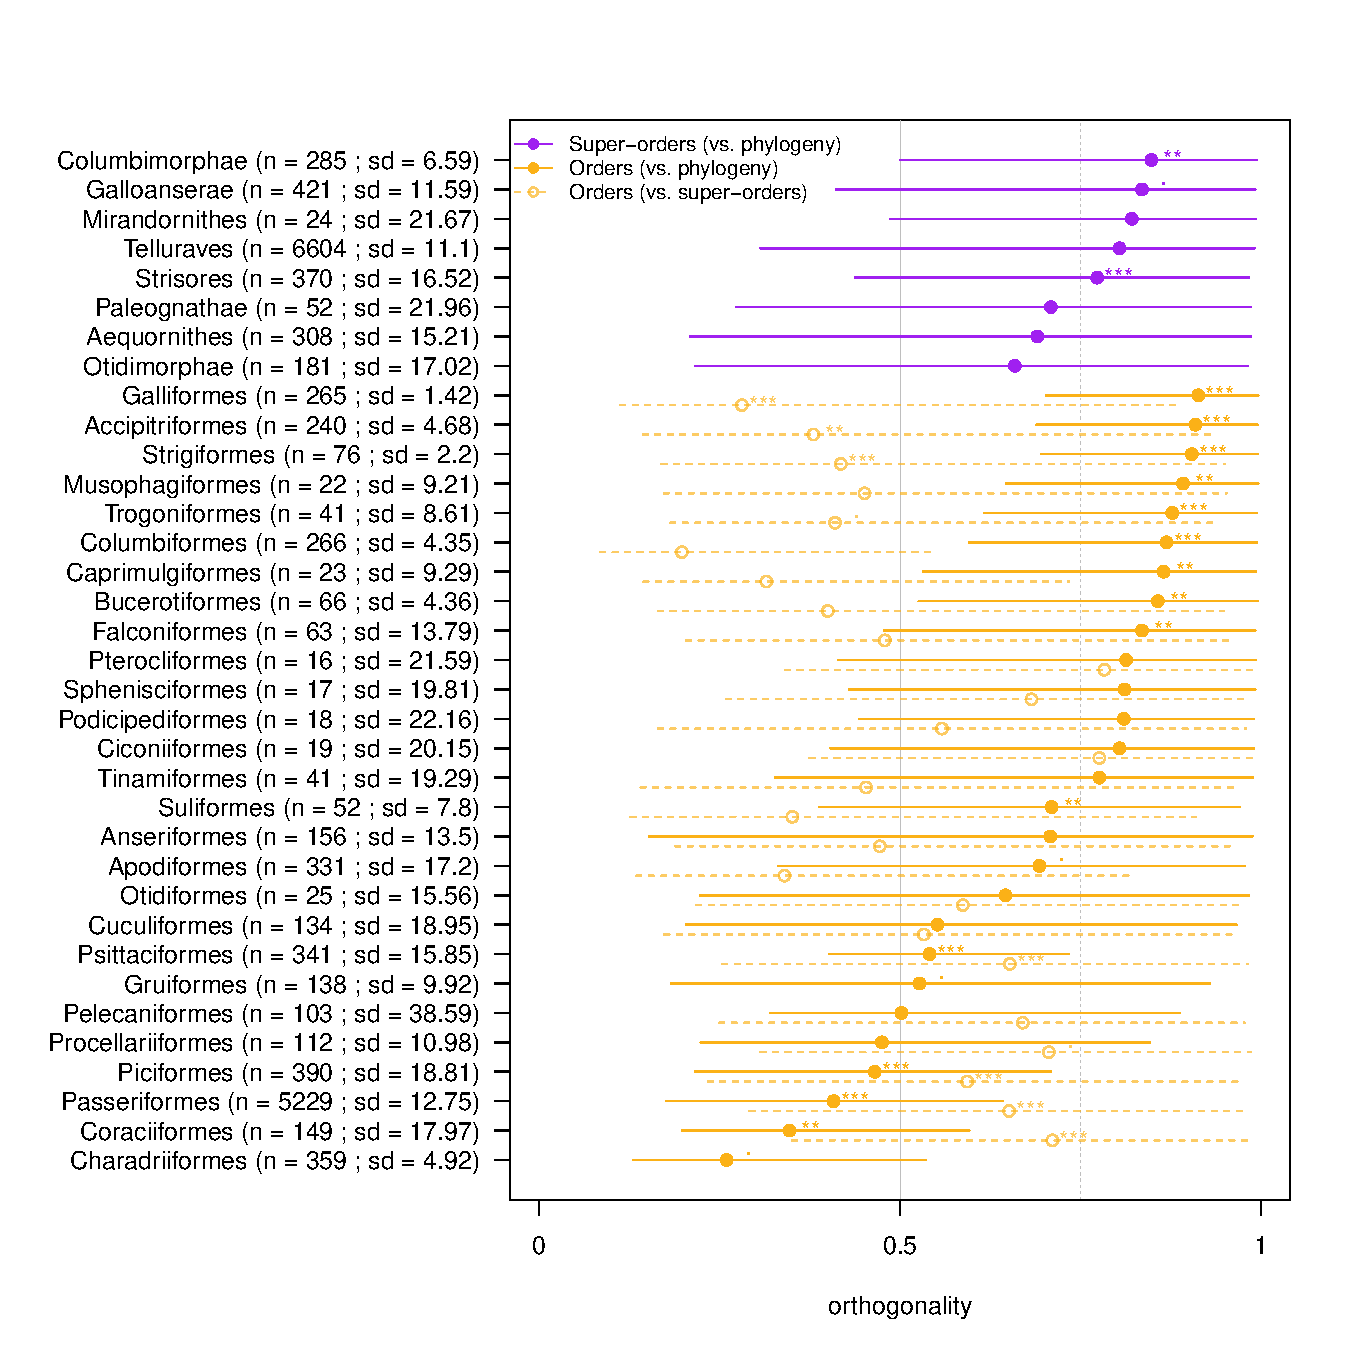
\includegraphics[width=0.9\textwidth]{Figures/orthogonality_results.pdf}
% \caption{.}
% \label{Fig:orthogonality}
% \end{figure}

% \bigskip

% \noindent \textbf{Figure \ref{Fig:orthogonality}:}
% \textbf{Clade's orthogonality.}
% Orthogonality of each clade's major axis of phenotypic variation compared to their parent or parent's parent clade.
% Orthogonality is represented on the horizontal axis and scales from 0 (modulo of $0^\circ$) to 1 (modulo of $90^\circ$) with the background grey and dashed grey lines representing, respectively, an orthogonality of 0.5 (modulo of $45^\circ$) and 0.75 (modulo of $67.5^\circ$).
% Dots represent the median orthogonality of each clade and the lines their 95\% CI.
% No super-order's major axis of phenotypic variation is parallel to the global phylogenetic major axis (red lines and circles) and 12/25 orders are at least half orthogonal to the major axis of their super-order (green lines and circles).
% These results are even clearer when compared to the global phylogenetic major axis (green dashed lines and open circles) where only 3/25 are less than half orthogonal.
% We also indicate the number of species (n) and the standard deviation (sd) of their major axes of phenotypic variation orientation over the 4000 variance-covariance posteriors (sd; expressed in degrees).
% For each clade we also measured the posterior probability of each clade's orientation being different from their parent's clade or the global phylogenetic major axis relative to their sample size and sd.
% The stars represent the posterior probability of the clade's orientation being different from the comparison clade. (*** = pp $> 0.99$; ** = pp $>0.95$; * = pp $> 0.9$; . = pp $> 0.8$).
% Only two out of six super-orders; 6/25 orders relative to their super-order and 9/25 orders relative to the phylogeny have a pp $> 0.99$.
% This is the result of the variation in sample size (n) and standard variation (sd) among clades. 
% A companion plot showing further nested structure within the Passeriformes is shown in Fig. S\ref{fig_orthogonality_passeriformes}.

% \bigskip


Evolutionary innovation can arise in any direction in trait space.
Although the global phylogenetic major axis of phenotypic variation aligns closely with the first dimension of the raw shapespace (70.96\% of the global phylogenetic major axis of phenotypic variation is aligned with PC1; Fig. \ref{Fig:ellipses}), no super-order, and only seven of the 27 orders (Procellariiformes, Pelecaniformes, Charadriiformes, Coraciiformes, Psittaciformes and Passeriformes), are aligned mainly with PC1 (Fig. \ref{Fig:ellipses}-bar plots); innovation dominates at this scale.
This pattern of orthogonality also holds for sub-orders and families within the Passeriformes where only half of the sub-orders (Meliphagoidea, Corvides and Passerida) and seven of the 23 families (Eurylaimides, Meliphagoidea, Petroicidea, Fringilidae, Aegithaloidea, Pyconotiae, Nectariniidae) align with the Passeriformes major axis of phenotypic variation (Fig. S\ref{fig_ellipses_passeriformes}).
In addition to the lack of alignment of clade major axes of phenotypic variation with the phylogenetic major axis, we also found that within clades, phenotypic variation is either highly constrained (varying almost entirely along a single axis; e.g. in Galliformes) or higher-dimensional than expected (there is no clear dominant major axis; e.g. in Podicipediformes) from the global phylogenetic major axis of phenotypic variation.
For example, Accipitriformes (hawks and allies) have major axes of phenotypic variation that mainly align with the second dimension of the shapespace suggesting distinct directions of evolution for the clade relative to the global phylogenetic level but uniformity in their beak shape within the clade.
In contrast, the Podicipediformes (grebes) are highly variable across all dimensions suggesting that all components of the shapespace are necessary to describe their beaks.
These observations illustrate multiple routes to innovation and imply that within clades species can evolve in many directions (akin to Endler \textit{et al}.'s \cite{endler2005animal} random innovation) or follow a single direction (akin to Endler \textit{et al}.'s \cite{endler2005animal} specific innovation) and that reorientations of trait space can arise in any direction, in any lineage, and at any time throughout avian history.


\section*{Species elaborate, clades innovate}

The disconnect between observations of reorientation of trait space at the clade level and a dominance of elaboration at the species level could be viewed as a paradox.
We formalise this paradox by testing whether elaboration is more common at higher taxonomic levels than at the species level.
We compared the area under the curve of the scaled density of elaboration and innovation at both the species level and the clade level.
We then measured the difference between both areas and found that there was a significant difference in innovation among species and clades but no clear difference in elaboration (Fig. \ref{Fig:relative_EI}).
This difference confirms our observation that while innovation is common and perhaps even dominant at the clade level, elaboration dominates at the species level. So, although species evolve preferentially along a shared major axis of phenotypic variance, this major axis changes frequently among clades.
However, we suggest that rather than a paradox the reorientation of trait space can instead arise as a result of small innovations that arise in a common direction among closely-related species.
This idea is similar in concept to multiple adaptive peak models where species evolve in a heterogeneous adaptive landscape and share similar responses to selection pressures within adaptive zones \cite{hansen1997stabilizing}.
This implies that gradual directional evolution \cite{pagel2022general}, rather than exceptional megaevolutionary jumps \cite{venditti2011multiple,cooney2017mega}, may be sufficient to explain diversity in avian beak morphology.

% \begin{figure}[!htbp]
% \centering
%    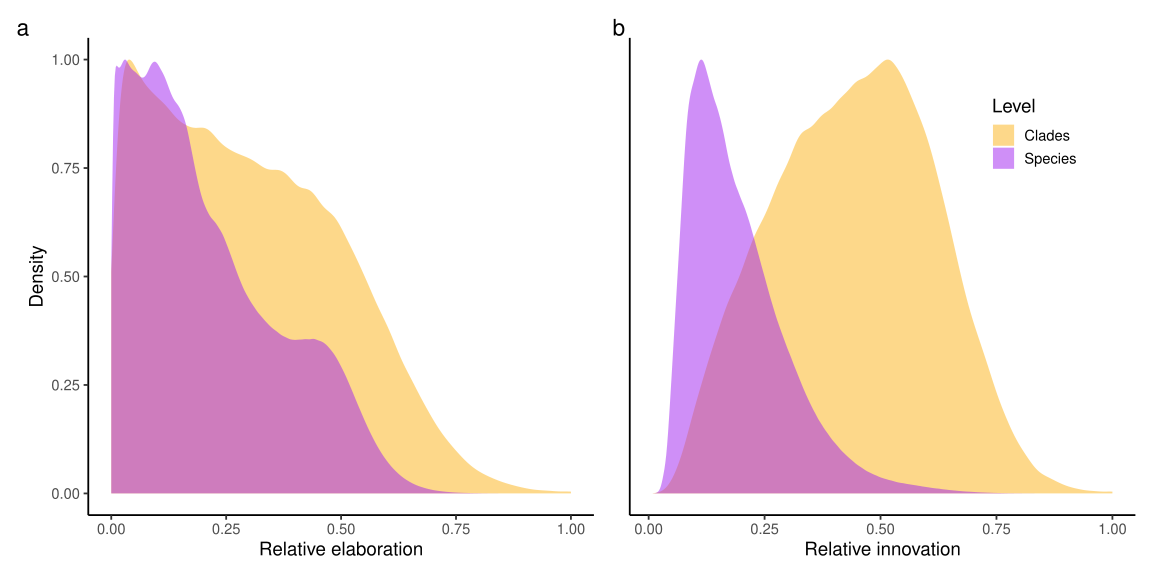
\includegraphics[width=0.9\textwidth]{Figures/relative_EI_gg_style.pdf}
% \caption{.}
% \label{Fig:relative_EI}
% \end{figure}

% \bigskip

% \noindent \textbf{Figure \ref{Fig:relative_EI}:} Comparisons of relative elaboration and innovation among clades (illustrated in figure \ref{Fig:ellipses}) and among species (figure \ref{Fig:phylogeny}).
% a) the elaboration (blue) for each species in each 4000 posterior samples compared to the elaboration for each of the 35 clades (yellow).
% The scores for each clade are scaled by the maximum score within the clade (corresponding to the scaled ellipses in figure \ref{Fig:ellipses}) and the scores for species are scaled by the maximum species elaboration score.
% This allows us to compare elaboration in species and clades despite their different sample sizes.
% We use the Bhattacharryya coefficient (BC) to quantify the overlap of the area under the curve for species and clades. 
% For elaboration the overlap is BC = 0.217, indicating no distinguishable dissimilarity in the amount of elaboration across the posterior samples between species or clades. 
% b) the same as a) but using innovation score. 
% For innovation the overlap has BC = 0.039, which indicates a clear difference in the amount of innovation across the posterior samples between species and clades.


% Paragraph 8: conclusion
\section*{Conclusions}

Our results show that although at the species-level most bird beaks are elaborating along a megaevolutionary major axis of phenotypic variation, at the macroevolutionary level innovation away from the global phylogenetic major axis of phenotypic variation is much more common. 
This nested structure of elaboration at a lower (species) taxonomic level and innovation at a higher (clade) taxonomic levels could thus explain the diversity of bird beaks we observe today.
However, individual species-level variation in the past could also have led to a shift in a clade's line of least evolutionary resistance through different evolutionary routes on a dynamic adaptive landscape. 
Taken together, our results suggest that the signature of evolutionary reorientations in deep-time (innovation), coupled with elaboration at the species-level, is a robust explanation of the massive diversity of bird beaks we observe today and is consistent with recent suggestions that apparently abrupt phenotypic shifts observed in univariate analyses can be explained by gradual Darwinian processes \cite{pagel2022general, BurinWhales,goswami2022}.
Indeed, the global phylogenetic major axis of phenotypic variation is an emergent property of reorientation of trait space among clades that requires no special evolutionary process: megaevolutionary patterns appear to be an inevitable outcome of evolution on a shifting adaptive landscape. 



% \section*{Methods}


% \textbf{Beak shape data.}
% We used the dataset from \cite{cooney2017mega,hughes2022global,chira2020signature} which consists of four landmarks and three curves of 25 semi-landmarks each, taken from 3D scans of  the beaks of 8748 bird species.
% The landmark data were aligned with Procrustes superimposition using the R package \texttt{Morpho} \cite{Rcore,Morpho} and we removed the size component and controlled for symmetry (see \cite{cooney2017mega,hughes2022global,chira2020signature} for detailed descriptions of data collection and processing).
% We ordinated the superimposed landmarks using a principal components analysis (PCA) and selected the eight first dimensions of the resulting PCA.
% These eight dimensions contained at least 95\% of variance in each super-order, and 98.7\% of the variance in the whole dataset.
% We used a threshold of $>95$\% of variance explained for each super-order because although the overall distribution of the variance on each PC axis in the whole trait-space is decreasing (i.e.
% $\sigma$ PC1 $<$ $\sigma$ PC2 $<$ $\sigma$ PC3), this is not always true for each super-order.
% For example, in the Mirandornithes, PC2, then PC4, and then PC1 contained the most variance (Fig. \ref{Fig:ellipses} and S\ref{Fig:axes_variance}).
% This protocol for selecting the number of PC axes ensures that the resulting trait-space contains enough variance for each super-order (see Fig. S\ref{Fig:axes_variance}).
% This procedure resulted in an $8748 \times 8$ matrix that contains at least 95\% of the variance in all observed living bird beaks (hereafter, the shapespace).

% \textbf{Phylogenetic data.}
% We used a random subsample of 1000 trees from the avian tree distribution of \cite{jetz2012global} for the analyses and the one randomly selected tree for the figures (Fig. \ref{Fig:phylogeny}).
% We pruned these trees to contain only the 8748 species present in our beak shapespace.

% \textbf{Phylogenetic GLMM analysis.}
% We ran a Bayesian phylogenetic generalised linear mixed model (pGLMM) using the \texttt{MCMCglmm} and \texttt{ape} R packages \cite{MCMCglmm, ape} with the shapespace data as a multidimensional response variable, the error in the dataset as residuals, and each clade's phylogeny as a nested random term, i.e., a model of:

% \begin{equation}
% \text{shapespace} \mathtt{\sim} \text{residuals(shapespace)} + \text{random(phylogeny)}
% \end{equation}

% This model allows us to estimate a phenotypic variance-covariance matrix for each clade and the phylogeny as a whole, and one for the residuals in the shapespace itself \cite{robinson2013quantifying}.
% These variance-covariance matrices were then used in a base projection-rejection analysis to measure the elaboration and innovation scores (see below).
% We ran two separate nested models.
% The first model used one random term for the global phylogeny and 35 nested random terms, one for each super-order and order containing more than 15 species in our dataset (Fig. \ref{Fig:ellipses}).
% This resulted in a multidimensional GLMM with a $8748 \times 8$ response variables, one global residual term and 36 random terms.
% The second model was fitted to a subset of the dataset containing only the 5229 Passeriformes species with 30 nested random terms, one for each sub-order and families containing more than 15 species in our dataset (Fig. S\ref{fig_ellipses_passeriformes}.
% This resulted in a multidimensional GLMM with a $5229 \times 8$ response variables, one global residual term and 30 random terms.
 
% To account for phylogenetic uncertainty we ran the model using different tree topologies from the tree distribution in \cite{jetz2012global}.
% Because of the very large size of our model and dataset, however, running the full model on multiple trees was computationally unfeasible (it would require 2 CPU years and 4TB of RAM for each of the models, i.e. the global phylogeny and the Passeriformes models).
% Instead, we developed and implemented a ''mini chains'' MCMCglmm method using the R package \texttt{mcmcmglmmm} \cite{mcmcmcglmmm}.

% \textbf{mcmcmcglmmm.}
% This method runs relatively short Monte-Carlo Markov chains (MCMC) across a large number of different phylogenetic trees and concatenates the resulting short posteriors into one larger posterior distribution that contains the phylogenetic uncertainty information.
% We performed the method using the following protocol (see Fig. S\ref{Fig:mcmcmcglmm}).
% First we ran three independent MCMCglmm chains (hereafter the parameterisation chains) for 50k generations with the trait data and the model described above on the consensus tree from the tree distribution, along with flat priors with a belief parameter of 2\%, i.e. with a very low weight on the priors;
% Next we extracted the following parameters from the parameterisation chains:
% a) the conservative burnin average time across the three chains, defined as the highest number of iterations required to first reach the median posterior likelihood value multiplied by 1.1; and
% b) the mini-chains priors, defined as the median posterior model values from the parameterisation chains with a belief parameter of 5\%.
% We then ran 400 mini chains in parallel with the estimated burnin time and priors to run 10 samples past the burnin.
% This resulted in 10 exploitable posterior samples for each tree.
% We used 400 trees because that was the number of models required to reach an effective sample size (ESS) of at least 200 for all the estimated parameters (see Fig. S\ref{Fig:model_ess_all_birds} and S\ref{Fig:model_ess_passeriformes}).
% Using this approach, we reduced the computational time to around 45 CPU hours and 9GB of RAM per mini-chain - a 400 fold improvement.
% The total analysis took around three CPU years using the shARC cluster from the University of Sheffield.
% Code to reproduce the procedure is available in the \href{https://raw.rawgit.net/TGuillerme/mcmcmcglmmm/main/inst/MCMCglmm_mini_chains.html}{\texttt{mcmcmcglmmm} vignette} \cite{mcmcmcglmmm}.

% \textbf{Elaboration/innovation scores using projection/rejection analyses.}
% We used the distributions of the 4000 posterior variance-covariance matrices to run the projection/rejection analyses to obtain  elaboration and innovation scores for bird beaks.
% We can use multilinear algebra to interpret elaboration and innovation \textit{sensu} \cite{endler2005animal} by using the major axis of the variance-covariance matrices as the ''line of least resistance'', or, specifically here, the line of elaboration for each random term (corresponding to the elaboration axis for each clade) and project either species or another major axis of phenotypic variation onto that clade.
% In brief we can then interpret where a species or a clade falls on the major axis of phenotypic variation of reference as its elaboration score, and how far a species is from that major axis of phenotypic variation as its innovation score.
% We calculated the elaboration and innovation scores using two main approaches:
% 1) by clades (i.e. to measure the elaboration/innovation among clades) where we calculated the projections of the major axes of each clade onto the global phylogenetic major axis of phenotypic variation (Fig. \ref{Fig:ellipses});
% and 2) by species (i.e. to measure the elaboration/innovation within clades) where we calculated the projections of each species onto a) the global phylogenetic major axis of phenotypic variation and b) the major axis of phenotypic variation of their specific clade (Fig. \ref{Fig:phylogeny}).
% To make the results easier to interpret, we centered and scaled them onto the centre of the major axis of phenotypic variation of interest and made the elaboration values absolute.
% In this way, we can interpret an elaboration or innovation score within the 0-1 range to be non exceptional (i.e within the 95\% confidence interval of the variance-covariance matrix).
% The full mathematical procedure is described in detail in the supplementary materials (section \ref{supp_projection}).
% Code to reproduce the analyses is available at \href{https://raw.rawgit.net/TGuillerme/dispRity/master/inst/vignettes/Projection_analysis.html}{this \texttt{dispRity} vignette} % TODO: update link to release when releasing
% and implemented in the \texttt{dispRity} package \cite{dispRity}.

% \textbf{Clade orthogonality.}
% We measured the orthogonality of each random term (i.e. clade) in our models compared to their parent clade and their parent's parent clade.
% For example, the variance-covariance matrices of the Columbimorphae random terms against the phylogeny random terms, the Columbiformes random terms against the Columbimorphae random terms (parent) and the whole phylogeny random terms (parent's parent).
% To measure orthogonality we calculated the angles between the major axes of phenotypic variation of the focal clade and their parent clade for each posterior variance-covariance matrix as well as within each clade, by randomly comparing major axes of phenotypic variation within a clade.
% We converted each angle measurement into an orthogonality metric where 0 corresponds to flat angles ($0^\circ$ or  $180^\circ$) and 1 to right angles ($90^\circ$ or $270^\circ$).
% We then measured the posterior probability of the angles within a clade being different to the angles among clades.
% These results are available in Fig. \ref{Fig:orthogonality}.


\bibliographystyle{Science}
\bibliography{references}

\section*{Acknowledgements}
We acknowledge IT Services at The University of Sheffield for the provision of the High Performance Computing Service.
We thank M. Adams, H. van Grouw, R. Prys-Jones and and Zo\"{e} K. Varley from the Bird Group at the NHM, Tring.
We are indebted to the volunteer citizen scientists at http://www.markmybird.org for helping to build the database of bird beak shape and contribute to our understanding of avian evolution. 
\textbf{Funding.}
This work was funded by the European Research Council (615709 Project ‘ToLERates’), UKRI-NERC Grant NE/T000139/1 and a Royal Society University Research Fellowship (URF R 180006 to G.H.T.).
\textbf{Author contributions.}
G.H.T., A.P.B., N.C., and T.G. designed the study. J.A.B., C.R.C., E.C.H., and G.H.T. % and Z.K.V.
curated the data. T.G. analysed the data. All authors contributed to the writing of the manuscript.
\textbf{Competing interests.}
We declare no competing interests.
\textbf{Data an materials availability.}
The raw and processed data used in this analysis is available from \href{https://figshare.shef.ac.uk/account/articles/21526146}{figshare} \cite{fighsaredata}.
The code used to reproduce the figures and tables is available from \href{https://github.com/TGuillerme/elaboration_exploration_bird_beaks}{GitHub} \cite{githubrepo}.


\section*{Supplementary materials}
Methods\\
Supplementary material 1: glossary\\
Supplementary material 2: additional results\\
Supplementary material 3: Passeriformes results\\
Supplementary materials 4: detailed projection and rejection operations\\
Figs. S1 to S8\\
Table S1\\


% TODO: Add list of supplementary materials
% All this comes after the references
% Figures and captions after this


\noindent \textbf{Figure \ref{Fig:phylogeny}:}
The avian phylogeny (n = 8748 species) coloured by species beak shape innovation and elaboration level.
Blue and yellow colours on the branches of the phylogeny highlight species with relatively low distances to the global centroid of trait space whereas orange to red colours indicate high distance from the centroid.
Innovation and elaboration scores are represented concentrically in a nested fashion with the most external pairs of circles (innovation and elaboration bands) representing comparisons for each species at the order level, then at the super-order level, and finally at the global phylogenetic level.
The boxplots at the bottom of the figure summarise the distribution of the median innovation and elaboration values for all levels (bottom left), showing that elaboration is more common than elaboration,
and the pooled median innovation and elaboration values for all three different levels (bottom right), showing that elaboration and innovation is more common at higher taxonomic levels than at the order level.
We can observe an increase in the distance of species to the global centroid of trait space at deeper phylogenetic scales with greater distances generally composed of more elaboration than innovation.
A companion plot showing further nested structure within the Passeriformes is shown in Fig. S\ref{fig_phylogeny_passeriformes}. 

\noindent \textbf{Figure \ref{Fig:ellipses}:}
Panel A) shows ellipses representing the scaled average posterior variance-covariance response from the pGLMM models for each super-order (coloured ellipses) compared to the global (all birds) phylogenetic component of the models (grey ellipses).
We scaled the ellipses so the length of the major axis of phenotypic variation of the clade ellipse is the same length as that of the global phylogenetic major axis ellipse (in eight dimensions).
The first inset ellipse plot shows the positions of all super-order ellipses relative to the global phylogenetic ellipse.
Subsequent inset plots show the results for each super-order. 
Inset barplots show the proportion of variance associated with each of the eight PC axes in shape morphospace.
The inset boxplots correspond to the elaboration (E) and innovation (I) scores for all 4000 posterior samples.
The dots represent the median elaboration and innovation values while the thick and dashed lines represent the 50\% and 95\% confidence intervals respectively.
These scores were calculated on the unscaled ellipses resulting in different scales of elaboration and innovation for each plot.
Panel B) shows the results for each order.
A companion plot showing further nested structure within the Passeriformes is shown in Fig. S\ref{fig_ellipses_passeriformes}.


\noindent \textbf{Figure \ref{Fig:orthogonality}:}
\textbf{Clade's orthogonality.}
Orthogonality of each clade's major axis of phenotypic variation compared to their parent or parent's parent clade.
Orthogonality is represented on the horizontal axis and scales from 0 (modulo of $0^\circ$) to 1 (modulo of $90^\circ$) with the background grey and dashed grey lines representing, respectively, an orthogonality of 0.5 (modulo of $45^\circ$) and 0.75 (modulo of $67.5^\circ$).
Dots represent the median orthogonality of each clade and the lines their 95\% CI.
No super-order's major axis of phenotypic variation is parallel to the global phylogenetic major axis (red lines and circles) and 12/25 orders are at least half orthogonal to the major axis of their super-order (green lines and circles).
These results are even clearer when compared to the global phylogenetic major axis (green dashed lines and open circles) where only 3/25 are less than half orthogonal.
We also indicate the number of species (n) and the standard deviation (sd) of their major axes of phenotypic variation orientation over the 4000 variance-covariance posteriors (sd; expressed in degrees).
For each clade we also measured the posterior probability of each clade's orientation being different from their parent's clade or the global phylogenetic major axis relative to their sample size and sd.
The stars represent the posterior probability of the clade's orientation being different from the comparison clade. (*** = pp $> 0.99$; ** = pp $>0.95$; * = pp $> 0.9$; . = pp $> 0.8$).
Only two out of six super-orders; 6/25 orders relative to their super-order and 9/25 orders relative to the phylogeny have a pp $> 0.99$.
This is the result of the variation in sample size (n) and standard variation (sd) among clades. 
A companion plot showing further nested structure within the Passeriformes is shown in Fig. S\ref{fig_orthogonality_passeriformes}.

\noindent \textbf{Figure \ref{Fig:relative_EI}:} Comparisons of relative elaboration and innovation among clades (illustrated in figure \ref{Fig:ellipses}) and among species (figure \ref{Fig:phylogeny}).
a) the elaboration (blue) for each species in each 4000 posterior samples compared to the elaboration for each of the 35 clades (yellow).
The scores for each clade are scaled by the maximum score within the clade (corresponding to the scaled ellipses in figure \ref{Fig:ellipses}) and the scores for species are scaled by the maximum species elaboration score.
This allows us to compare elaboration in species and clades despite their different sample sizes.
We use the Bhattacharryya coefficient (BC) to quantify the overlap of the area under the curve for species and clades. 
For elaboration the overlap is BC = 0.217, indicating no distinguishable dissimilarity in the amount of elaboration across the posterior samples between species or clades. 
b) the same as a) but using innovation score. 
For innovation the overlap has BC = 0.039, which indicates a clear difference in the amount of innovation across the posterior samples between species and clades.

\begin{figure}[!htbp]
\centering
    \includegraphics[width=0.9\textwidth]{Figures/InnovElabTree_main_text_with_box.pdf}
\caption{.}
\label{Fig:phylogeny}
\end{figure}

\begin{figure}[!htbp]
\centering
   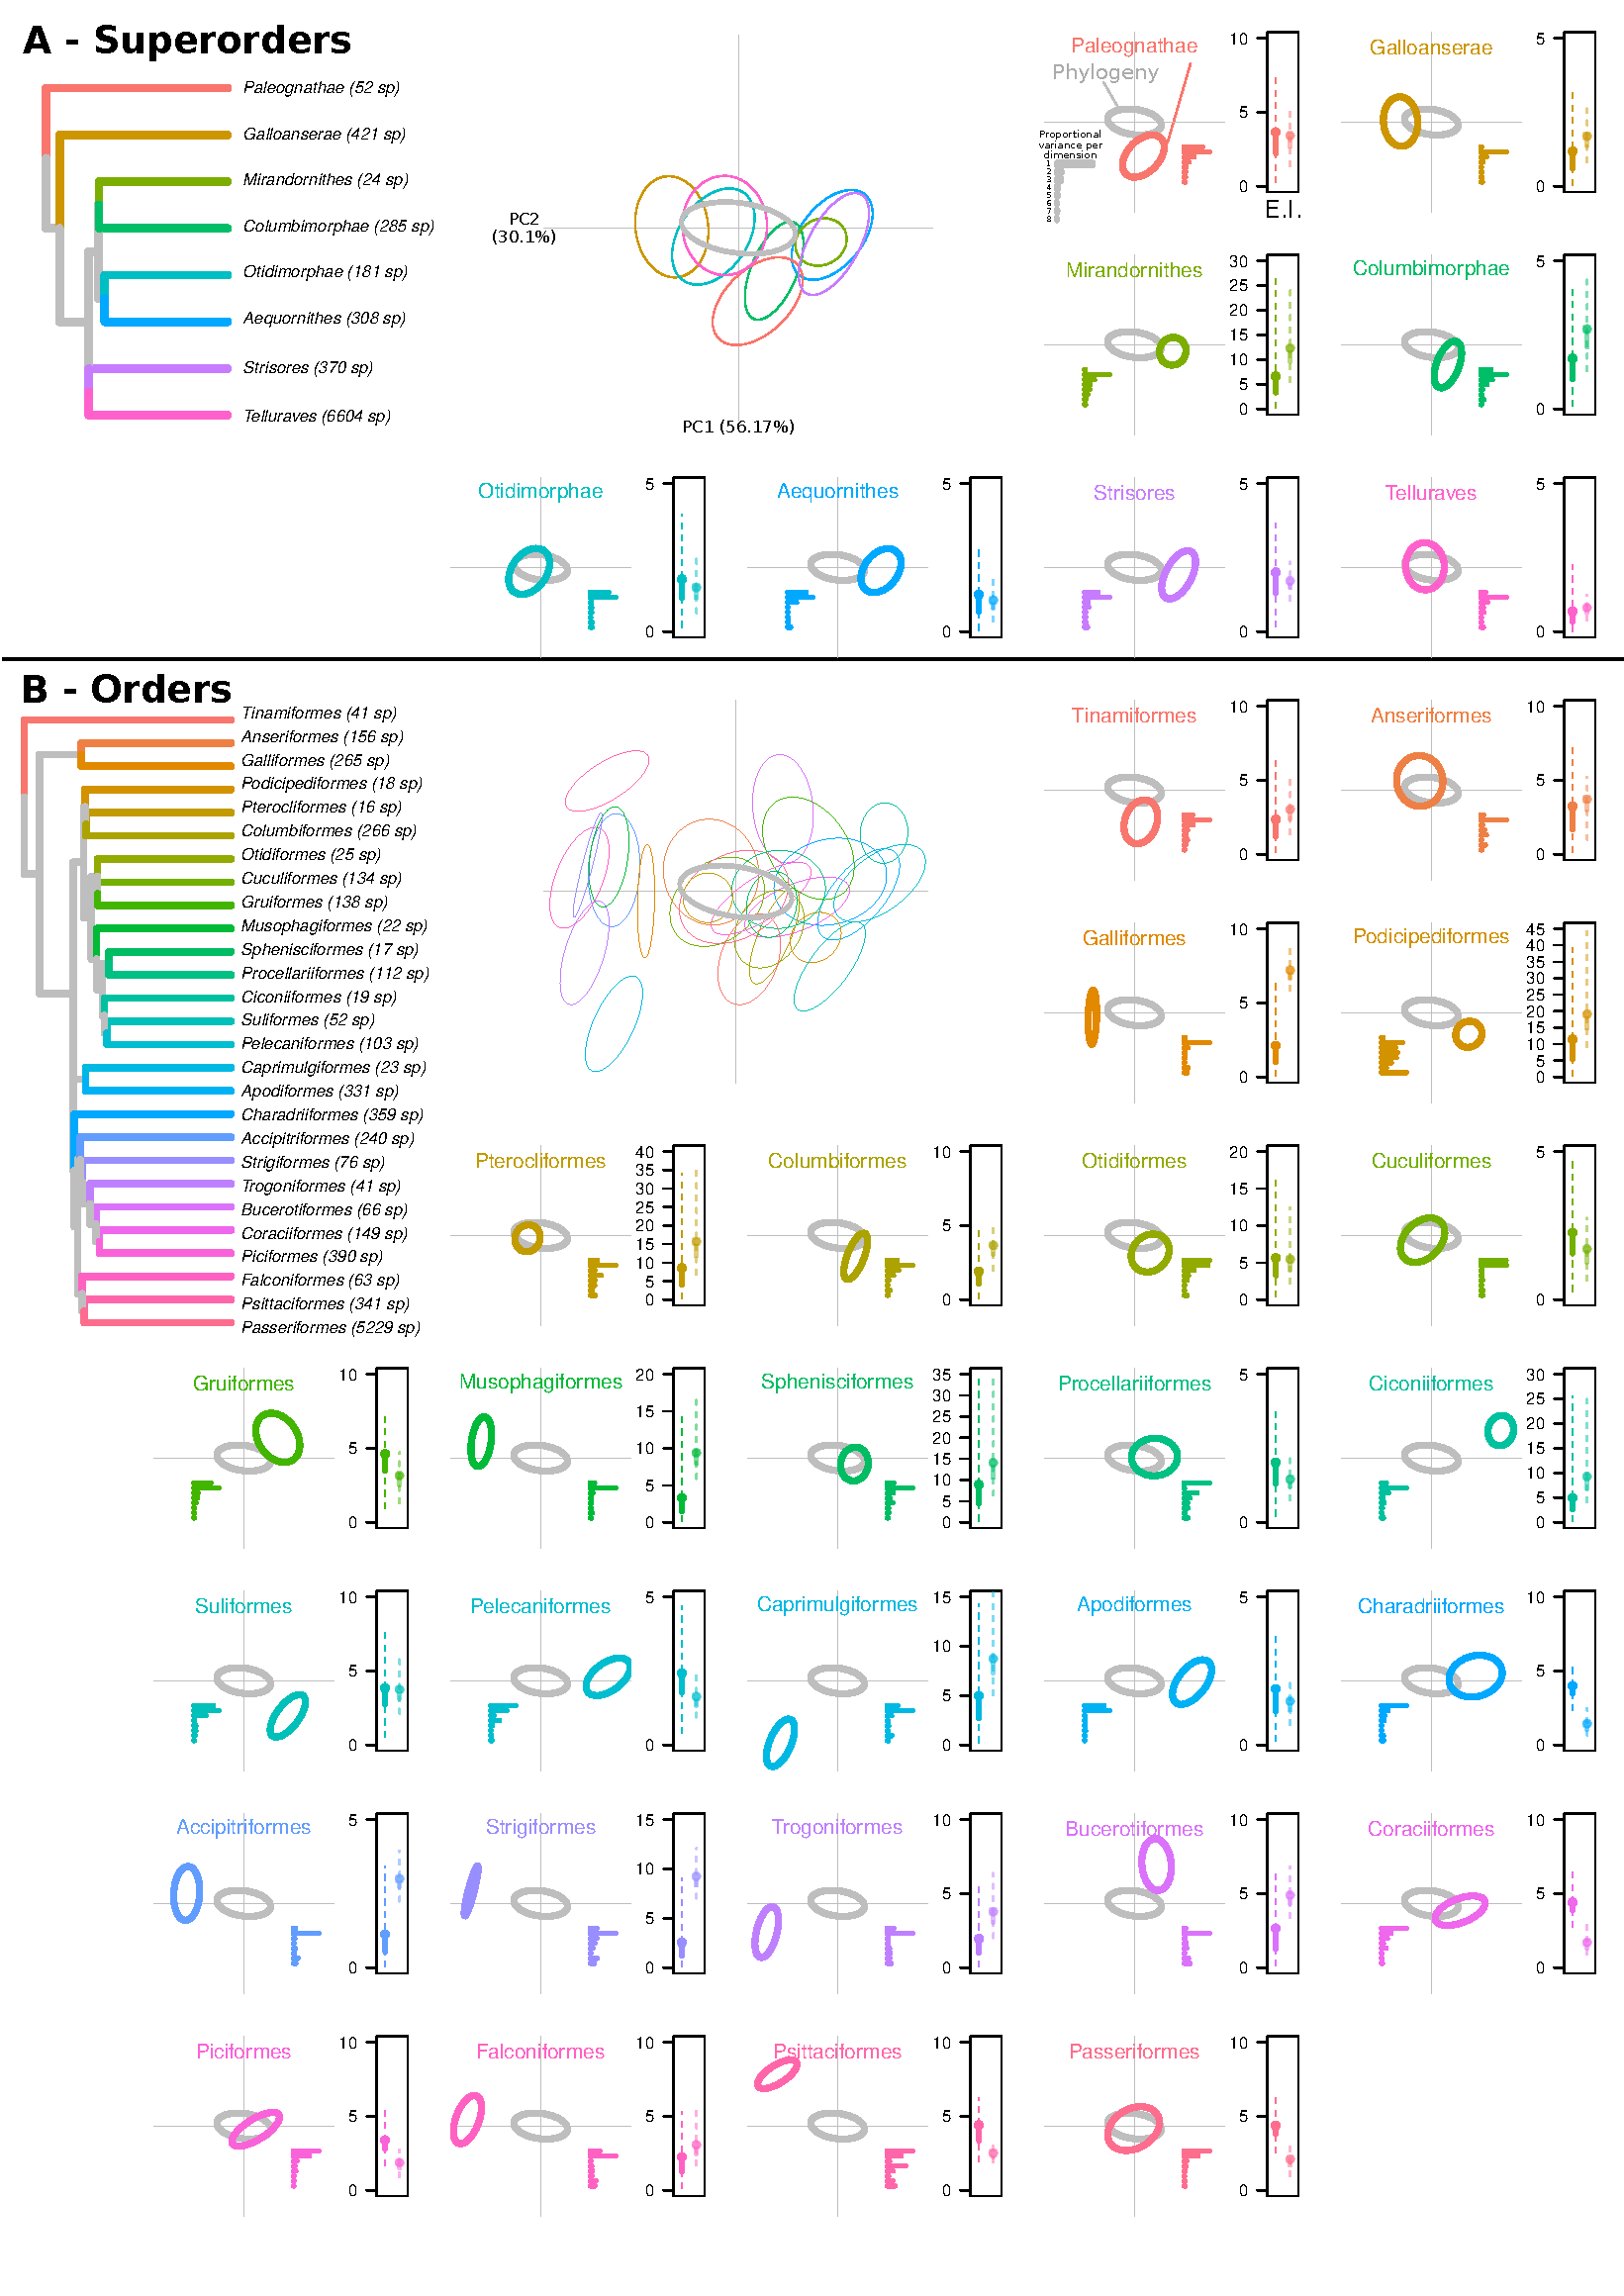
\includegraphics[width=1\textwidth]{Figures/ellipses.pdf}
\caption{.}
\label{Fig:ellipses}
\end{figure}

\begin{figure}[!htbp]
\centering
   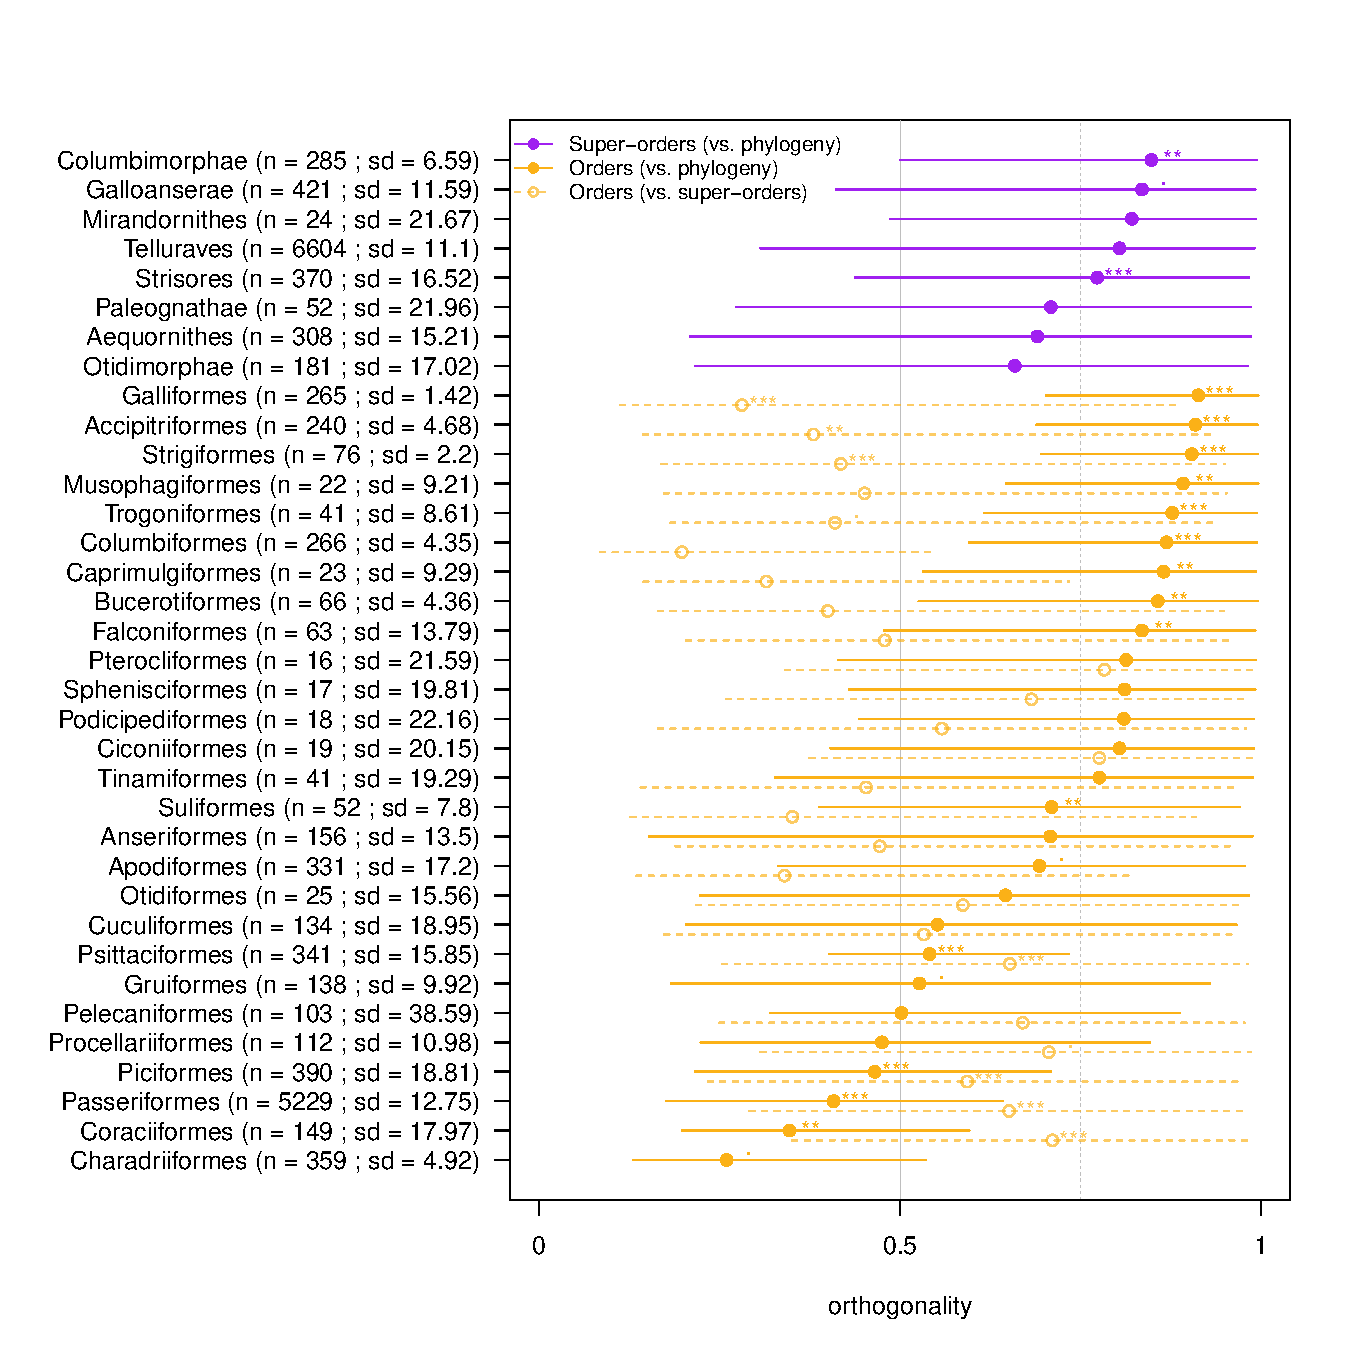
\includegraphics[width=0.9\textwidth]{Figures/orthogonality_results.pdf}
\caption{.}
\label{Fig:orthogonality}
\end{figure}

\begin{figure}[!htbp]
\centering
   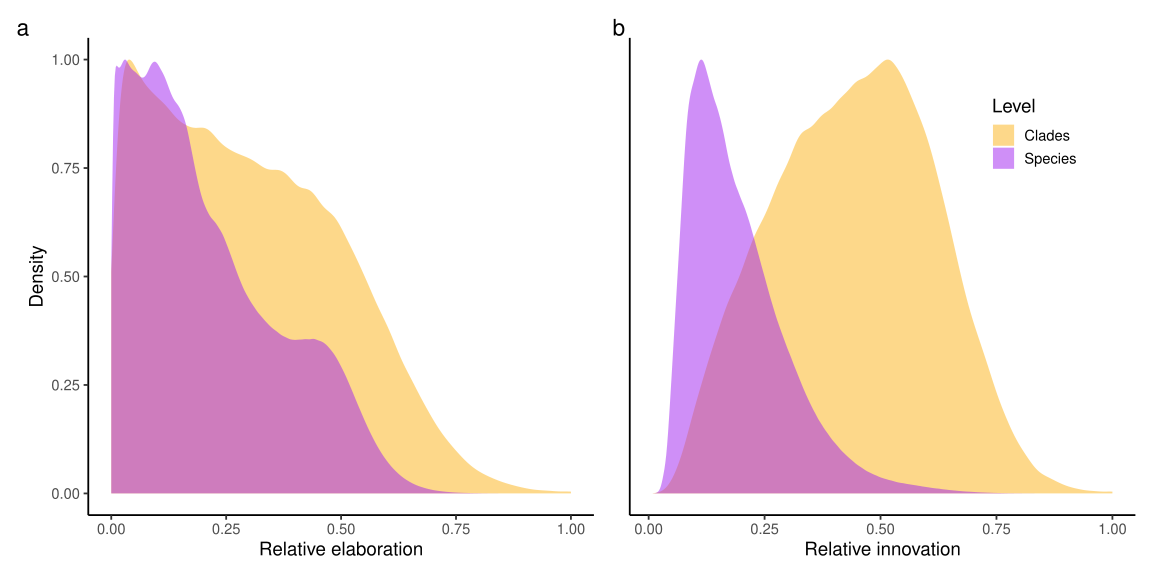
\includegraphics[width=0.9\textwidth]{Figures/relative_EI_gg_style.pdf}
\caption{.}
\label{Fig:relative_EI}
\end{figure}


\end{document}